\chapter{Виды и механизмы перестрахования. Пропорциональное перестрахование, квотный договор. Уравновешенность договора, экономические и финансовые условия}
\problem{}
Нарисовать кривую Лоренца для распределения Парето с $F(x) = 1 - (x/\sigma)^{-\alpha},$ $x \geq \sigma > 0$.
\solution{}

    Найдем квантильную функцию распределения $F$:
    \begin{equation}
        y = 1 - (x/\sigma)^{-\alpha}  \; \Rightarrow \; x = \sigma(1 - y)^{-\frac{1}{\alpha}},
    \end{equation}
    \begin{equation}
        \int_0^u \sigma(1-t)^{-\frac{1}{\alpha}}dt = \int_{1-u}^1 \sigma s^{-\frac{1}{\alpha}}ds = \sigma \frac{\alpha - 1}{\alpha}\left(1 - (1 - u)^{\frac{\alpha - 1 }{\alpha}}\right).
    \end{equation}
    Следовательно 
    \begin{equation}
        L_X(u) = 1 - (1 - u)^{\frac{\alpha- 1}{\alpha}}.
    \end{equation}
    См Рис \ref{fig:hw8t1p1}.

    \begin{figure}[htbp]
        \centering
        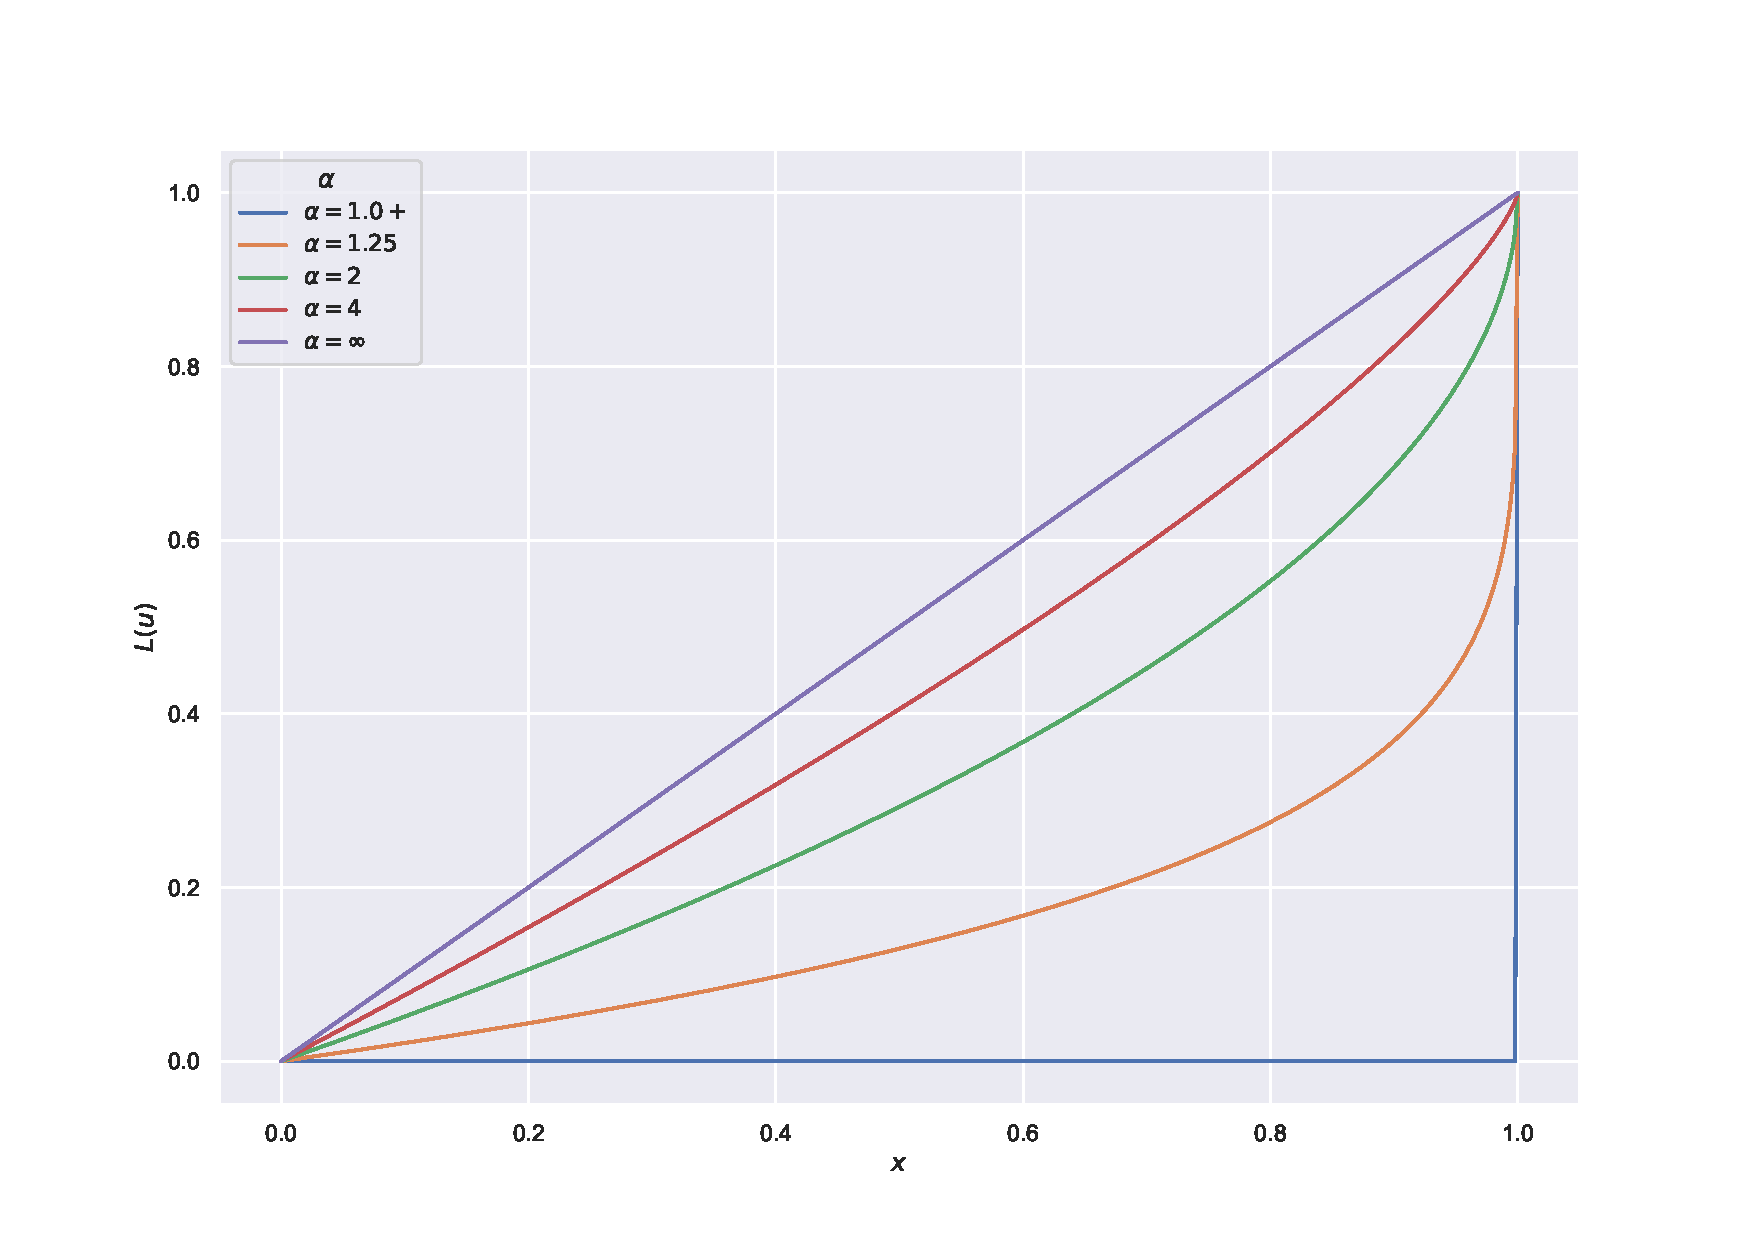
\includegraphics[width=\linewidth]{pics/hw8t1p1.pdf}
        \caption{Кривая Лоренца для распределения Парето с разными параметрами}
        \label{fig:hw8t1p1}
    \end{figure}

\problem{}
Проверить, что если $X \prec_{Lor} Y$, то $CV(X) \leq CV(Y)$. Верно ли обратное утверждение?
\solution{}

$$X \prec_{Lor} Y \iffdef \frac{X}{\E[X]} <_{cx} \frac{Y}{\E[Y]}$$
Имеем: 
\begin{align}
    & \E [X^2] / (\E [X])^2 \leq \E[Y^2 ]/ (\E[Y])^2, \\
    & (\E[X^2] - (\E[X])^2)/ (\E[X])^2 \leq (\E[Y^2] - (\E[Y])^2) / (\E[Y])^2.
\end{align}
Взяв квадратный корень от обех частей получаем требуемое утверждение.
Чтобы показать, что обратное неверно, возьмем случайные величины $X,Y$ со средним, равным $1$, $X<C=const$ п.н., $Y$ - неограничена, и $\var X > \var Y $. Подойдут например $X: \P(X=0) = 2/3, \P (X = 3) = 1/3$ и $Y \sim Exp(1).$ Тогда $\sqrt 2 = CV(X) > CV(Y) = 1 $. Но $\E(X - 3)^+ = 0 < \E(Y - 3)^+ = e^{-3}$. Значит, либо $X<_{cx} Y$ либо $X$ и $Y$ - несравнимы. 

\problem{}
Пусть $X$ и $Z$ - независимые случайные величины, $X \sim \Gamma(1, \lambda^{-1})$, $Z \sim \Gamma(\alpha, 1)$. Проверить, что $Y = X/Z$ имеет распределение Парето с функцией распределения $F(x) = 1 - (x/\sigma)^{-\alpha},$ $x \geq \sigma > 0$.
\solution{}

\begin{multline*}
    \iint_{x/y \leq t} f_{X,Y}(x,y)dxdy = \iint_{x/y \leq t} f_{X}(x) f_Y(y)dxdy =\\= \left[x/y = u, x = v \right] =
    \int_{u\leq t}\int_{v \in \mathbb R}f_X(v)f_Y(v/u)\frac{|v|}{u^2}dvdu =\\= 
    \int_{0\leq u\leq t}\int_0^{+\infty} \frac{1}{\lambda}e^{v/\lambda} \frac{1}{\Gamma(\alpha)}\left( \frac{v}{u}\right)^{\alpha - 1} e^{-v/u} \frac{v}{u^2} dv du =\\= 
    \int_{0\leq u\leq t}\frac{1}{\Gamma(\alpha) u^{\alpha +1} \lambda}\int_0^{+\infty} v^\alpha \exp\left\{-\left(\frac1\lambda + \frac1u\right)v\right\} dv du =\\= 
    \int_{0\leq u\leq t}\frac{(\frac1\lambda + \frac1u)^{-(\alpha +1)}}{\Gamma(\alpha) u^{\alpha +1} \lambda}\int_0^{+\infty} s^\alpha \exp\left(-s\right) ds du =\\= \frac{\Gamma(\alpha + 1)}{\lambda\Gamma(\alpha)} \int_{0\leq u\leq t} \left(\frac u\lambda + 1 \right)^{-\alpha - 1}du = \alpha \int_1^{1+ t/\lambda} s^{-\alpha - 1}ds = \\ = 1 - (1 + t/\lambda)^{-\alpha}.
\end{multline*}

\problem{}
Показать, что $ X <_{st} Y \not\Rightarrow X <_k Y $. (Указание: рассмотреть $X \sim U(0, 2)$, $Y \sim U(1, 2)$, где $U(a, b)$ - равномерное
распределение на $(a, b)$.)
\solution{}
Рассмотрим предложенные случайные величины. $X^* = X/\mathbb E[X] = X, Y^* = Y/\mathbb E [Y] = \frac{2}{3}Y$. Для любого $t$ $F_X(t)\geq F_Y(t) \iff X<_{st} Y$. Однако, $\frac{2}{3}Y \sim U(2/3, 4/3)$ и $\mathbb E[(X^* - 4/3)^+] = 1/3 > \mathbb E [(Y^* - 4/3)^+] = 0$. Следовательно, $X^*$ и $Y^*$ либо несравнимы, либо $Y^* <_{sl} X^*$. Осталось вспомнить, что $Y^* <_{sl} X^* \Leftrightarrow Y <_{k} X_{k}$.

\problem{}
Показать, что $X <_k Y \not\Rightarrow X <_{st} Y$. (Указание: рассмотреть $X \sim Exp(1)$, $Y \sim Exp(2)$, где $Exp(a)$ - показательное
распределение с параметром $a$.)
\solution{}
Рассмотрим предложенные случайные величины. $X^* = X/\mathbb EX = X, \; Y^* = Y/\mathbb E Y = 2 Y \sim X \Rightarrow X^*<_{sl} Y^*$, но $\bar F_Y(x) = e^{-2x} < e^{-x} = \bar F_X(x), \; x\geq 0 \Rightarrow Y<_{st}X$.

\problem{}
Проверить, что гамма-распределение с $\alpha \geq 1$ и равномерное имеют тип IFR.
\solution{}
\begin{enumerate}
    \item Случай гамма распределения. Для простоты будем рассматривать $1/\lambda(x)$. Необходимо показать, что $1/\lambda(x) $ - убывает по $x$. 
    \begin{multline}
        1/\lambda(x) = \left( \frac{\beta^\alpha x^{\alpha - 1}}{\Gamma(\alpha)} \right)^{-1} \int_x^\infty \frac{\beta^\alpha t^{\alpha - 1}}{\Gamma(\alpha)}e^{-\beta t} dt =\\= \left[ t - x = u, dt = du \right] = \int_0^\infty \left(\frac{u}{x} + 1\right)^{\alpha -1}e^{-\beta u} du
    \end{multline}
        не возрастает по $x$ при $\alpha \geq 1$.

    \item Случай равномерного распределения $U(a,b)$.
    \begin{equation}
        \lambda(x) =\frac{\frac{1}{b-a}}{1 - \frac{x - a}{b - a}} =  \frac{1}{b - x},
    \end{equation}
    Это выражение возрастает по $x$.
\end{enumerate}

\problem{}
Показать, что если $X_i <_{mor} Y_i$, $i \geq 1$, то $\min_i X_i <_{mor} \min_i Y_i$.
\solution{}

Напомним, что $F_{\min_i X_i} (x) = 1 - (1 - F(x))^n$. Действительно, $\P( \min_i X_i < x) $ означает, что хотя бы 1 из $X_i$ меньше либо равен $x$. Это тоже самое, что
    \begin{equation}
        \sum_{k =1}^n \mathbb{P}(X_{(k)} \leq x, X_{(k+1)} > x ) =  \sum_{k=1}^n \binom{n}{k} F^k(x)(1 - F(x))^{n-k} = 1 - (1 - F(x))^n.
    \end{equation}
    Отсюда, поскольку $\frac{1 - F_X(x)}{1 - F_Y(x)}$ убывает по $x$, то 
    \begin{equation}
        \frac{1 - F_{\min_i X_i}(x)}{ 1 - F_{\min_i Y_i}(x)} = \left( \frac{1 - F_X(x)}{ 1 - F_Y(x)} \right)^n
    \end{equation}
    убывает по $x$ и, следовательно, $\min_i X_i <_{mor} \min_i Y_i$.